\documentclass[a4paper,12pt]{article}
\usepackage[T2A]{fontenc}
\usepackage[utf8]{inputenc}
\usepackage[english, russian]{babel}
\usepackage{minted}
\usepackage{graphicx}
\usepackage{caption}
\usepackage{subcaption}

\newenvironment{longlisting}{\captionsetup{type=listing}}{}

\newenvironment{pseudolisting}
 {\begin{minipage}{\linewidth}\vspace*{\topsep}}
 {\vspace*{\topsep}\end{minipage}}

\begin{document}

\begin{titlepage}
  \begin{center}
    \large
     
    \textbf{Федеральное государственное автономное образовательное учреждение высшего образования}
    \vspace{0.5cm}
 
    НАЦИОНАЛЬНЫЙ ИССЛЕДОВАТЕЛЬСКИЙ УНИВЕРСИТЕТ \\ "ВЫСШАЯ ШКОЛА ЭКОНОМИКИ"
    \vspace{0.5cm}
     
    Московский институт электроники и математики имени А. Н. Тихонова 
     
    Программа "Прикладная математика"
    \vfill
     
     
    Нигматуллин Роман Максимович
    \vfill
 
    \textsc{Лаборатная работа}\\[5mm]
     
    {\LARGE Теория погрешностей и машинная арифметика\\[2mm]
    }
  \bigskip
     
    3 курс, группа БПМ203
\end{center}
\vfill
 

 
\hfill\begin{flushright}
  \textbf{Преподаватель:}\\
  Брандышев Петр Евгеньевич
\end{flushright}%
\vfill
 
\begin{center}
  Москва, 2021 г.
\end{center}
\end{titlepage}


\tableofcontents

\section{Расчет частичных сумм ряда}
\subsection{Формулировка задачи}
Дан ряд, надо найти сумму аналитически как предел частичных сумм, затем вычислить частичные суммы в зависимости от N и сравнить абсолютную погрешность и кол-во верных цифр в частичной сумме.
   $$S(N) = \sum_0^N a_n$$
   $$a_n = \frac{32}{n^2 +5n +6}$$

\subsection{Код на Python}

\begin{longlisting}
\inputminted{python}{series.py}
\end{longlisting}

\subsection{Графики точности результата}
\begin{figure}[H]
\centering
\begin{subfigure}{.5\textwidth}
  \centering
  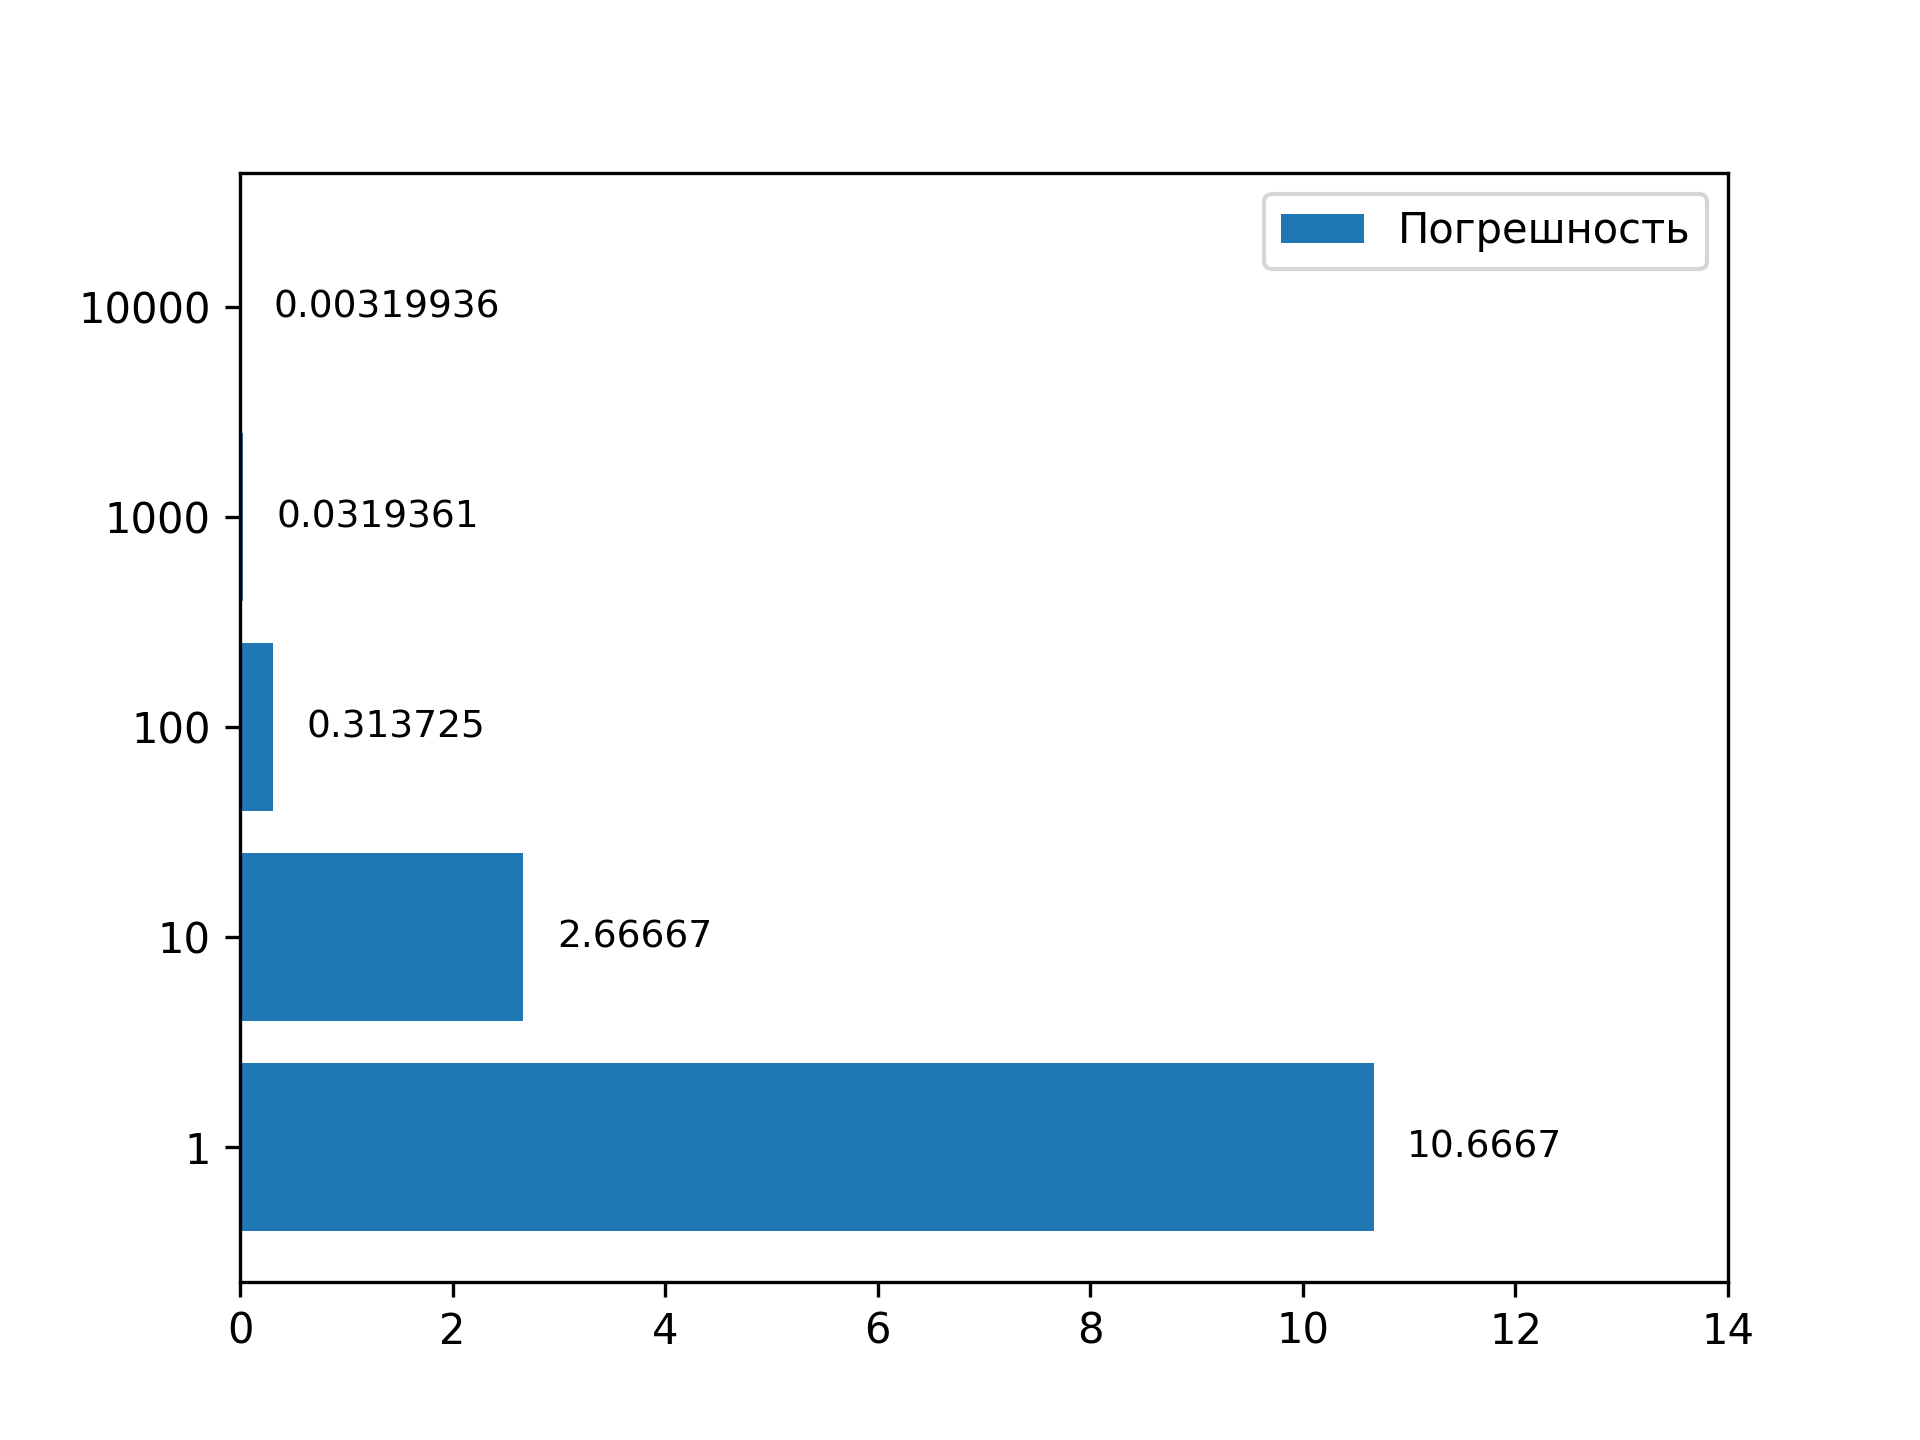
\includegraphics[width=\linewidth]{plots/series_error.png}
  \caption{Абсолютная погрешность}
  \label{fig:sub1}
\end{subfigure}%
\begin{subfigure}{.5\textwidth}
  \centering
  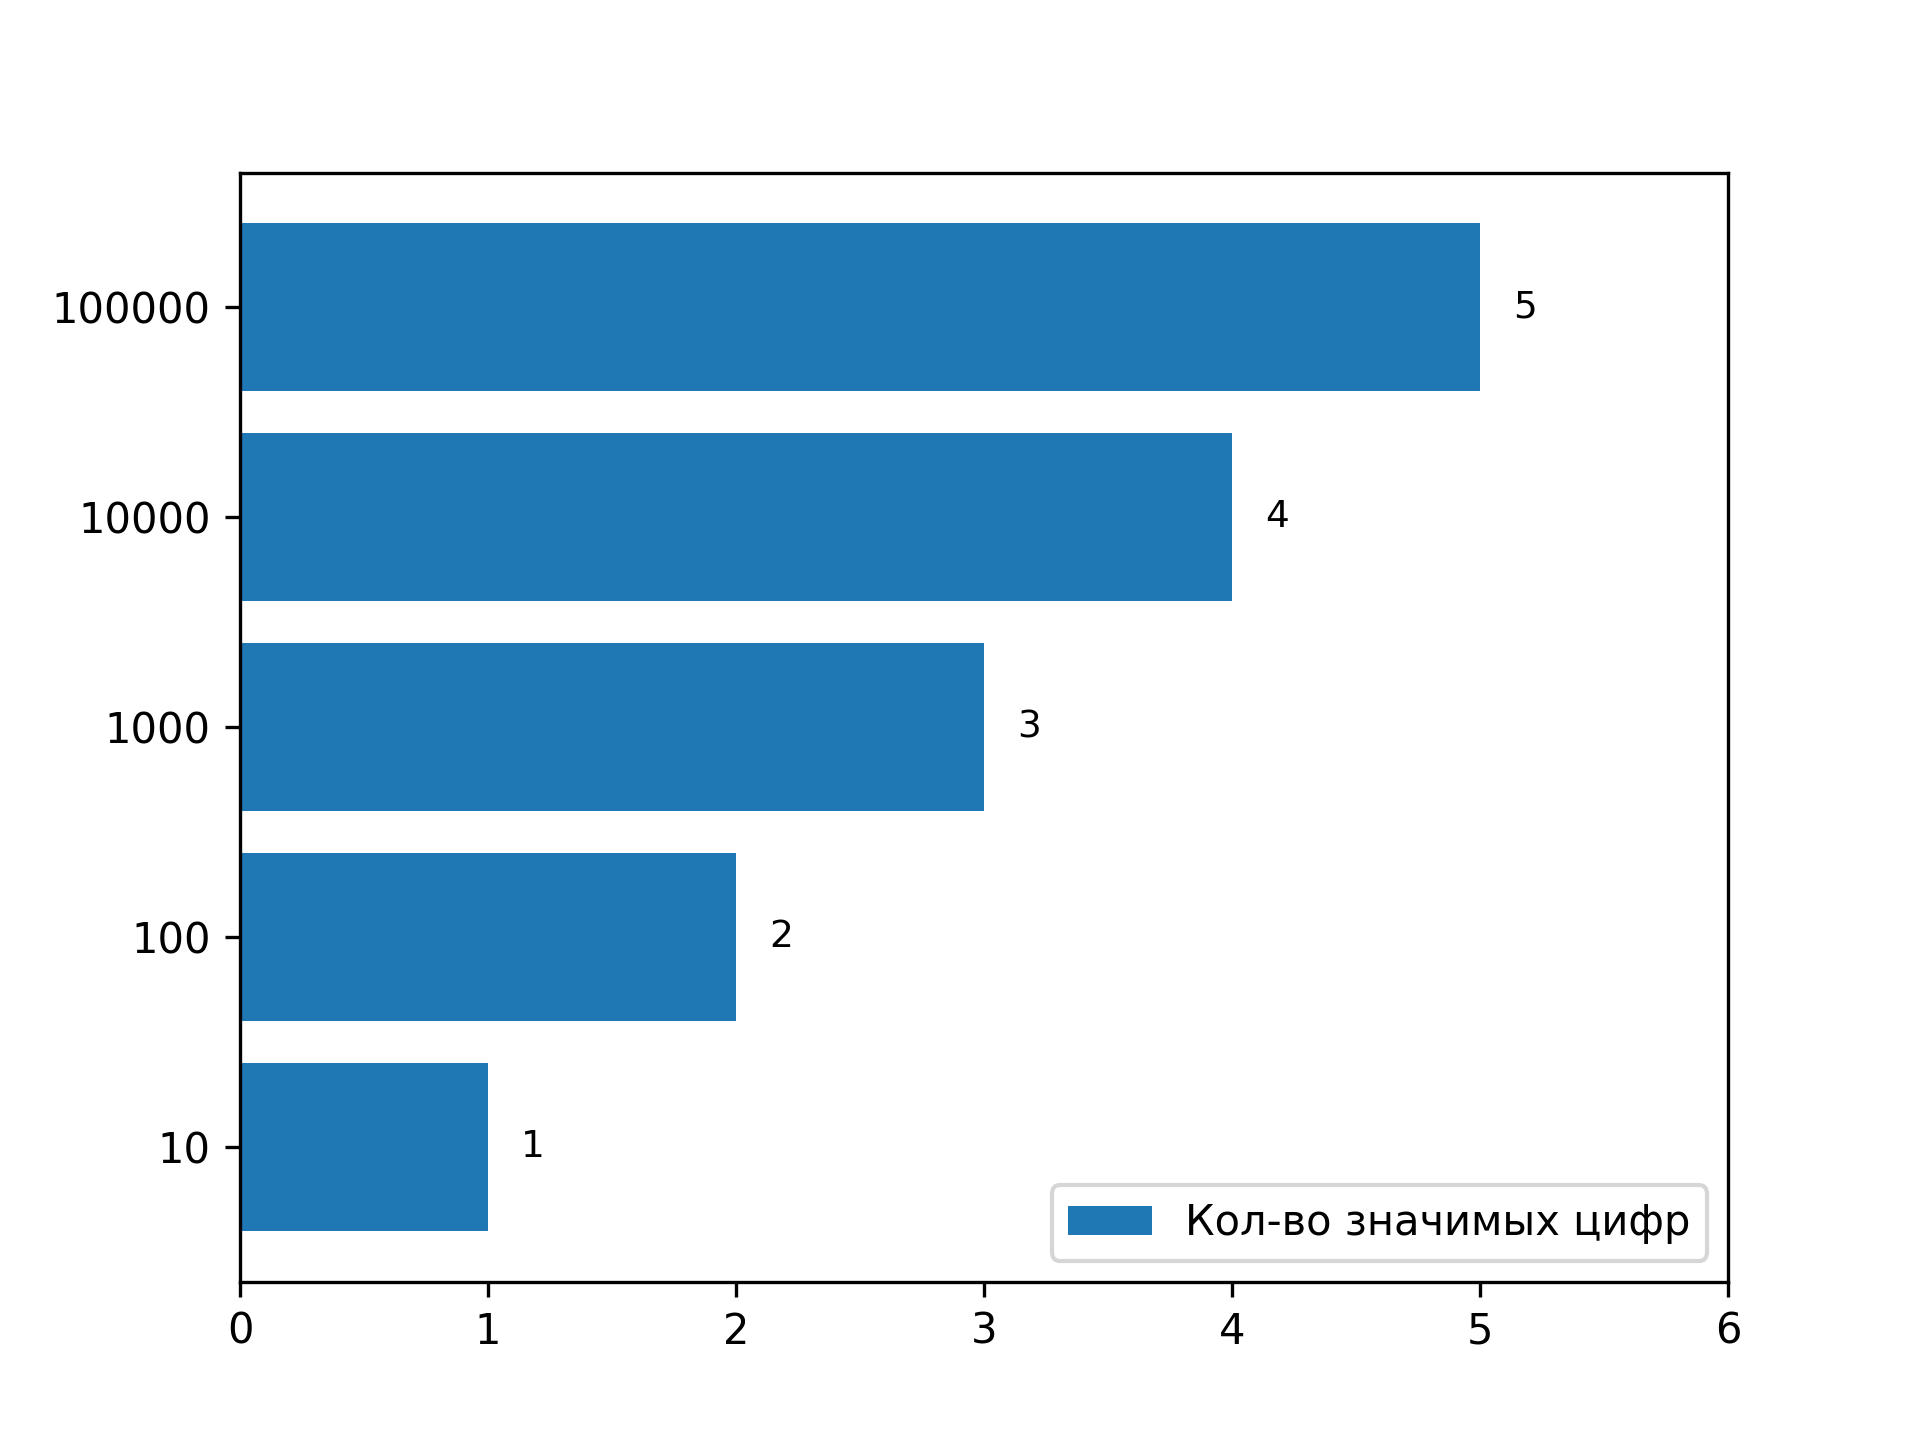
\includegraphics[width=\linewidth]{plots/series_n_digits.png}
  \caption{Кол-во значащих цифр}
  \label{fig:sub2}
\end{subfigure}
\caption{Точность в зависимости от N}
\label{fig:test}
\end{figure}

\section{Квадратное уравнение}
\subsection{Формулировка задачи}
Дано квадратное уравнение. Предполагается, что один из коэффициентов уравнения (помечен $*$) получен в результате округления. Произвести теоретическую оценку погрешностей корней в зависимости от погрешности коэффициента. Вычислить корни уравнения при нескольких различных значениях коэффициента в пределах заданной точности, сравнить.
    $$x^2+bx+c = 0$$
    $$ $$
   
\subsection{Код на Python}
\begin{longlisting}
\inputminted{python}{quadratic_eq.py}
\end{longlisting}

\section{Машинная точность}
\subsection{Формулировка задачи}
Вычислить значения машинного нуля, машинной бесконечности и машинного эпсилон в режимах одинарной, двойной и расширенной точности на двух алгоритмических языках.
\subsection{Код на Python}

\begin{longlisting}
\inputminted{python}{precision.py}
\end{longlisting}

\subsection{Код на C++}
\begin{longlisting}
\inputminted{c++}{precision.cpp}
\end{longlisting}


\section{Вычисления с ограниченной разрядностью}
\subsection{Формулировка задачи}
Составить программу, моделирующую вычисления на ЭВМ с ограниченной разрядностью $m$.
Решить задачу о вычислении суммы ряда для случая $n=10000$, используя эту программу. Составить график зависимости погрешности от количества разрядов $m = \{4, 5, 6, 7, 8\}$.

\subsection{Код на Python}

\begin{longlisting}
\inputminted{python}{series_fixed_precision.py}
\end{longlisting}

\subsection{Графики точности результата}
\begin{figure}[H]
\centering
\begin{subfigure}{.5\textwidth}
  \centering
  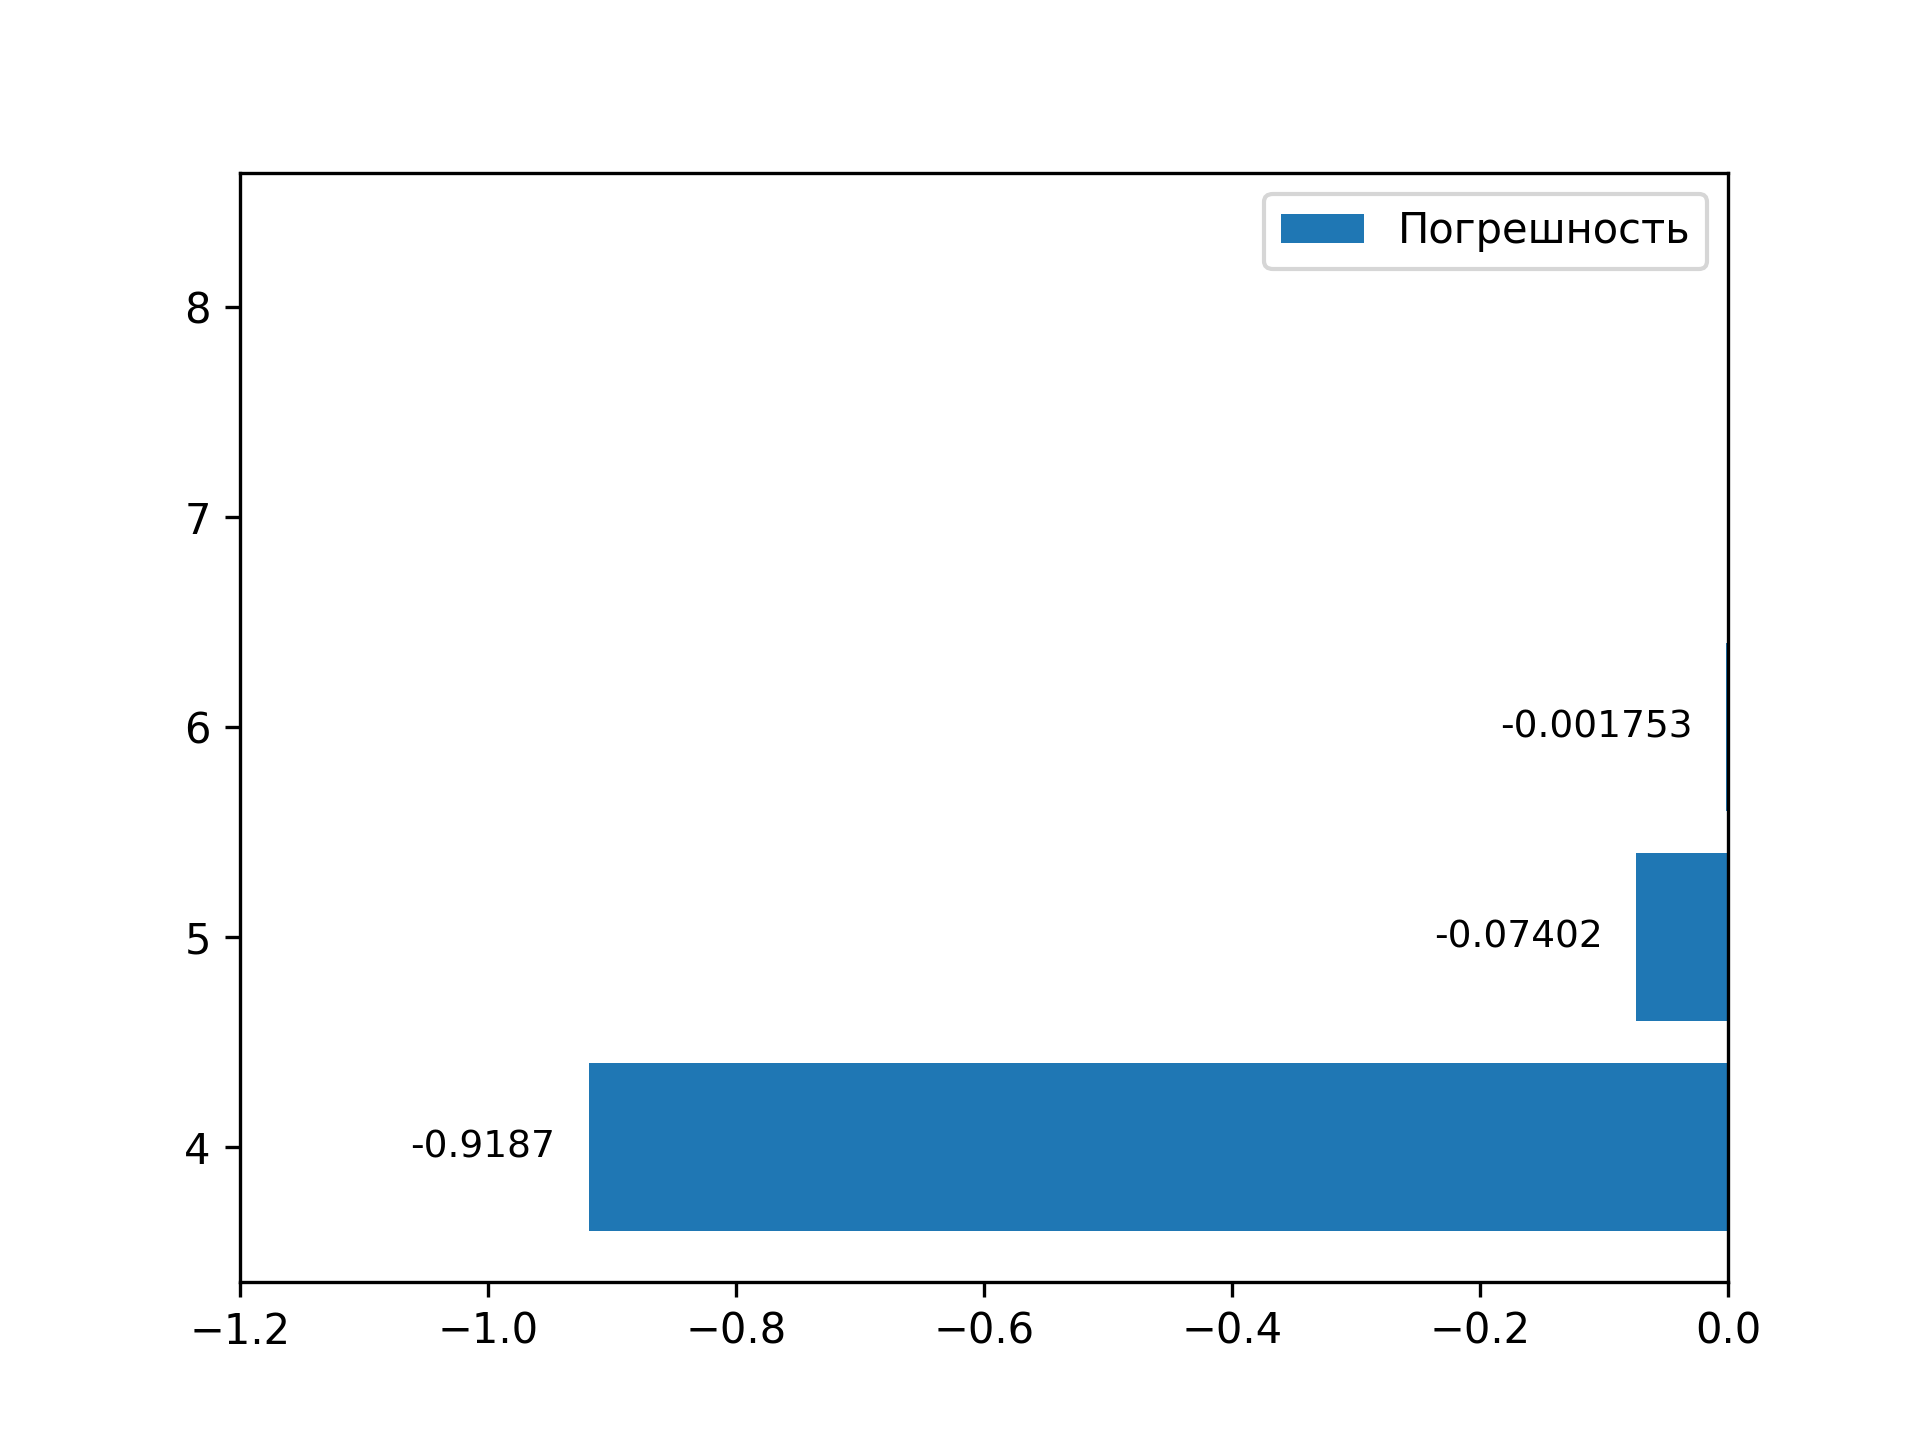
\includegraphics[width=\linewidth]{plots/series_fixed_error.png}
  \caption{Абсолютная погрешность}
  \label{fig:sub3}
\end{subfigure}%
\begin{subfigure}{.5\textwidth}
  \centering
  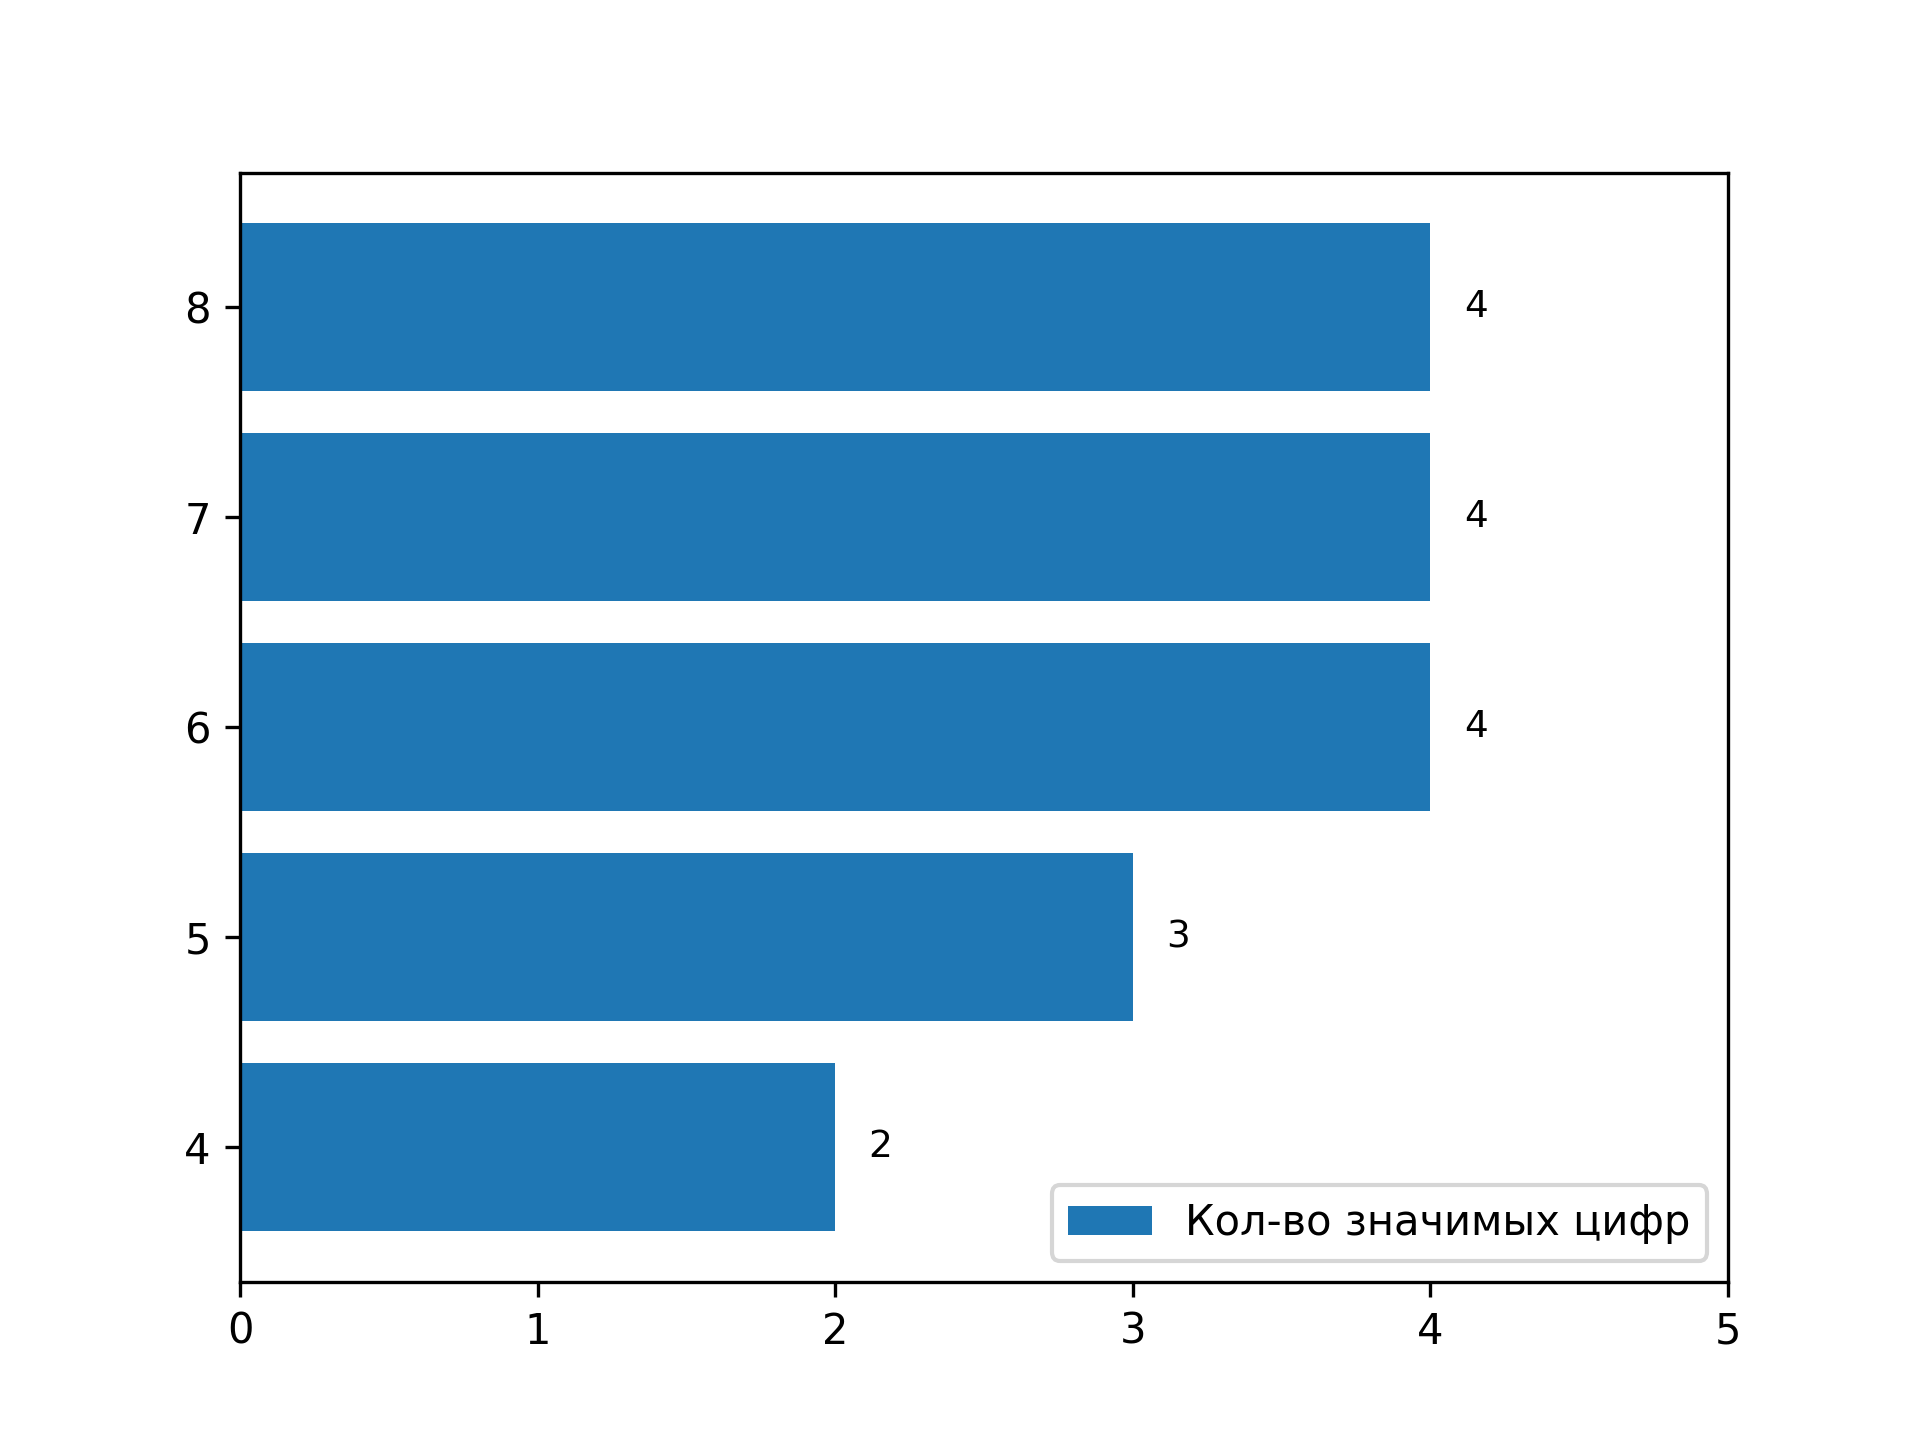
\includegraphics[width=\linewidth]{plots/series_fixed_n_digits.png}
  \caption{Кол-во значащих цифр}
  \label{fig:sub4}
\end{subfigure}
\caption{Точность в зависимости от разрядности}
\label{fig:test}
\end{figure}

\end{document}